\documentclass[conference]{IEEEtran}
\IEEEoverridecommandlockouts
\usepackage{amsmath,amssymb}
\usepackage{booktabs}
\usepackage{graphicx}
\IfFileExists{microtype.sty}{\usepackage{microtype}}{}
\usepackage{url}
\usepackage[hidelinks]{hyperref}
\IfFileExists{pcrr7t.tfm}{}{\renewcommand{\ttdefault}{cmtt}}

\newcommand{\dove}{\textsc{Dove}}
\newcommand{\dataset}{FinReason Cup 2026 Task~3}

\title{DOVE: Difference-Oriented Verification and Execution for Financial Numerical Verification}

\author{
\IEEEauthorblockN{Chenxu Zhao\textsuperscript{1,2}, Sichen Hui\textsuperscript{1,2}, and Qianqian Xie\textsuperscript{1,2,*}}
\IEEEauthorblockA{\textsuperscript{1}School of Artificial Intelligence, Wuhan University, Wuhan, China\\
\textsuperscript{2}Cognitive Language and Information Lab, Wuhan University, Wuhan, China\\
Team DOVE\\xqq.sincere@gmail.com}
\thanks{\textsuperscript{*}Corresponding author.}
}
\begin{document}
\bstctlcite{IEEEexample:BSTcontrol}
\maketitle

\begin{abstract}
Financial numerical verification requires selecting a reported fact and reconstructing its expected value from accounting evidence. We present DOVE (Difference-Oriented Verification and Execution), a deterministic system for FinReason Cup 2026 Task 3, and audit the reliability of its selection decisions. The system combines context-aware target selection with direct calculation, inverse calculation, sign recovery, and dimensional aggregation, and records operands, relationship coverage, and candidate scores in execution traces. The official Test submission achieves 655/680 correct answers (96.32\%), tying for eighth among 23 teams and solving all 464 DQC 0126 cases. Matched Practice comparisons on 332 examples yield 187 correct value pairs for DOVE, 25 for the organizer's full rule baseline, and 55 for fixed DOVE extraction followed by sign flipping. A factorial ablation identifies an interaction between weak aggregation and discrepancy-aware ranking. Reliability audits reveal a complementary result: fact-order changes alter up to 23 Test predictions, and a constructed incomplete competitor overturns all 30 correct reports in a controlled equation family. We report both the submitted system's performance and the selection mechanisms behind its reliability failures, separating numerical execution from evidence selection.
\end{abstract}

\begin{IEEEkeywords}
financial numerical verification, XBRL, rule-based systems, financial auditing, reliability audit
\end{IEEEkeywords}

\section{Introduction}
FinReason Cup 2026 Task~3 asks a system to locate a reported concept-period fact in an SEC EDGAR XBRL filing and reconstruct its expected value from the supplied evidence~\cite{xie2026overview,wang2026task3}. XBRL exposes numerical facts and accounting relationships, making rule-based execution a natural approach. The central difficulty is choosing what to execute: the same concept can occur in several financial scopes, and a relationship can be available even when some of its operands are missing.

We developed \dove{} (Difference-Oriented Verification and Execution) to address these choices through context-aware target selection and explicit numerical programs. The system selects among direct calculation, inverse calculation, sign recovery, and dimensional aggregation. Candidate scores combine relationship coverage, role support, conflicts, and discrepancy from the report. Execution traces retain the selected facts, operands, relations, and scores, connecting each output to the decision that produced it.

This paper presents the submitted competition system and a retrospective reliability audit. The official submission obtains 655/680 correct answers (96.32\%), including every DQC~0126 calculation-network case. Matched Practice comparisons show the contribution of numerical execution beyond sign reversal, while a factorial ablation identifies the joint effect of weak member aggregation and discrepancy-aware ranking. The audit then examines whether the same system preserves its outputs under fact permutations and selects a complete relationship when an incomplete competitor is available.

Reversing fact order changes 23 Test predictions without changing the underlying evidence. In a controlled equation family, discrepancy-aware ranking selects an incomplete relationship over a complete one for all 30 correct reports. These audits identify selection failures that precise arithmetic alone does not prevent.

Our contributions are an auditable rule-based competition system, matched Practice comparisons that separate extraction from subsequent execution, and reliability audits of order dependence and incomplete-candidate promotion. We describe the task and system, establish the evaluation protocol, and report task performance before examining reliability in Section~\ref{sec:reliability}.

\section{Task and Evaluation Contract}

\subsection{Task Formulation}
\label{sec:task}

Task~3 evaluates targeted numerical verification in organizer-packaged SEC EDGAR filings~\cite{xie2026overview,wang2026task3}. Each JSONL input record contains an \texttt{id} and a \texttt{query} string. The string embeds the task instructions, schema, presentation/calculation/definition/label linkbases, instance document, target-specific US GAAP taxonomy information, and two questions~\cite{task3baseline}. The questions specify a concept and period and request its reported and recomputed values. Both outputs must be derived from the supplied filing materials; an external service's existing data-quality findings are excluded by the task rules~\cite{task3submission}.

We represent the parsed task as
\begin{equation}
q=(c,\tau,\mathcal X), \qquad \hat z(q)=(\hat r,\hat y),
\end{equation}
where $c$ is the target concept, $\tau$ is an instant or duration, and $\mathcal X$ is the supplied filing and taxonomy evidence. The outputs $\hat r$ and $\hat y$ are the reported value and the value reconstructed from that evidence. Fact selection and program construction are specified in Section~\ref{sec:selection}.

An abbreviated starter-kit example uses the following target and period~\cite{task3baseline}:
\begin{quote}
\small\raggedright
\texttt{us-gaap:PaymentsToAcquire}\\
\texttt{PropertyPlantAndEquipment}\\
2021-09-01 to 2021-11-30.
\end{quote}
Its first question requests the reported amount; its second requests the amount derived from the supplied relationships. The public reference answer is
\begin{quote}
\small\ttfamily\raggedright
\{"extracted\_value": "-1284",\\
\phantom{\{}"calculated\_value": "1284"\}
\end{quote}
This reference pair illustrates the magnitude-preserving sign-recovery operation used by our system (Section~\ref{sec:programs}).

The submitted JSONL record additionally includes \texttt{id}; the evaluator judges the two-value answer object. The submission contract requires \texttt{"0"} when a value cannot be determined, so this token need not denote an observed financial zero~\cite{task3submission}.

The cases cover three DQC rules~\cite{dqcusrules}. DQC~0015 checks negative values for a specified concept list, with member exclusions that permit legitimate negative values. DQC~0117 compares reported totals with dimensional breakdowns in financial-statement hypercubes. DQC~0126 checks calculation consistency in financial-statement networks without an associated hypercube. These checks respectively motivate sign, dimensional, and calculation-network routes; their applicability conditions remain distinct.

The official evaluator assigns one label through successive checks~\cite{task3scoring,task3results}. An invalid two-key answer object receives S (structural error). Otherwise, a numerically incorrect reported value receives E (extraction error). Only after correct extraction can an incorrect recomputed value receive C (calculation error); matching both values receives A (accurate). Thus structural failure takes precedence over extraction, and extraction failure takes precedence over calculation. Numeric meaning is compared independently of formatting, with zero tolerance for the calculated value. For label counts $n_A,n_S,n_E,n_C$ and $V=n_A+n_S+n_E+n_C$,
\begin{equation}
\begin{aligned}
\mathrm{ACC}&=n_A/V, & \mathrm{SER}&=n_S/V,\\
\mathrm{EER}&=n_E/V, & \mathrm{CER}&=n_C/V.
\end{aligned}
\end{equation}
Here $V$ counts valid evaluator labels, including S; an invalid judge response is excluded. Missing case identifiers instead fail submission validation~\cite{task3submission}. The official Test used the organizer's LLM evaluator; our local Practice analyses use exact Decimal-normalized pair comparisons (Section~\ref{sec:protocol}).

\section{Related Work}
\label{sec:related}

\noindent\textbf{Financial numerical reasoning.}
FinQA studies multi-step financial question answering with annotated reasoning programs~\cite{chen-etal-2021-finqa}, while TAT-QA combines tabular and textual evidence with arithmetic operations~\cite{zhu-etal-2021-tat}. FinAuditing evaluates taxonomy-structured reasoning across related financial documents~\cite{wang2026finauditing}, and Herculean places financial reasoning within agentic workflows and tool use~\cite{peng2026herculean}. Financial language-model research also includes PIXIU and FinBen, which provide financial modeling resources and evaluation benchmarks~\cite{xie2023pixiu,xie2024finben}. MultiFinBen extends evaluation across languages and text, images, and audio~\cite{peng-etal-2026-multifinben}. AuditWen covers audit information extraction and question answering~\cite{jiajia-etal-2024-auditwen}, while AuditJudgLLM evaluates professional audit judgment~\cite{huang2027auditjudgllm}. FinTagging tests financial figure identification and linking to US GAAP concepts~\cite{wang2026fintagging}. Related domain-specific studies have examined biomedical language models and their evaluation~\cite{medicalfoundation,biomedicalsurvey}. These works advance domain-specific reasoning and evaluation, but targeted XBRL verification additionally requires selecting the correct accounting scope and an executable relationship with sufficient operands. DOVE addresses these requirements through context-aware fact selection and evidence-preserving numerical programs.

\noindent\textbf{XBRL validation.}
The XBRL US DQC publishes executable validation rules~\cite{dqcusrules,dqcimplementation}. Arelle provides context-aware fact access and calculation validation, and XULE supports business-rule execution, including DQC checks~\cite{arelle,xule}. These tools supply structured validation evidence. DOVE addresses the task-specific selection of a fact and reconstruction program to produce one numerical pair.

\noindent\textbf{Task-specific reference implementation.}
The organizer baseline extracts a concept-period fact and sums available calculation children with their weights, skipping missing children. When no sum is available, a negative fact with a debit or credit balance attribute triggers sign reversal; otherwise, it copies the report~\cite{task3baseline,task3rulecode}. We compare its full, extraction-only, and sign-flip modes with DOVE under the same local scoring protocol.

\noindent\textbf{Program-assisted computation.}
PAL and Program of Thoughts separate semantic reasoning from arithmetic by executing generated programs~\cite{pmlr-v202-gao23f,chen2023pot}. DOVE constructs programs through fixed rules over filing relationships, without language-model program generation at inference. Its audit examines the preceding evidence-selection decisions: exact execution preserves an incorrect scope choice or an incomplete operand set just as faithfully as a correct one.

\section{The Submitted DOVE System}
\label{sec:system}

\subsection{Overview and Evidence Representation}
\label{sec:overview}

\dove{} runs five stages: query and XBRL parsing, fact/context construction, target selection, candidate-program generation and ranking, and output with diagnostics. Parsing and evidence construction supply a common initial target-candidate list to the three prioritized routes in Figure~\ref{fig:overview}: eligible negative-fact selection, joint subtotal/program selection, and general target-first execution. The solver first checks for eligible negative facts. Otherwise, it attempts joint subtotal/program selection; if no joint pair is admitted, it uses general target-first execution. The joint route commits both a target and a program, while the other routes pass the selected target to program ranking. We use \emph{program family} for the arithmetic operation, direct calculation, inverse calculation, sign recovery, or dimensional aggregation, and \emph{route} for this control flow.

We use \emph{deterministic} to mean that a fixed configuration and identical ordered input yield the same output through fixed rules, scores, and tie breakers. Fact-order invariance is tested separately in Section~\ref{sec:order}.

\begin{figure*}[t]
\centering
% Editable vector source: figures/fig1_dove_architecture_solid.svg
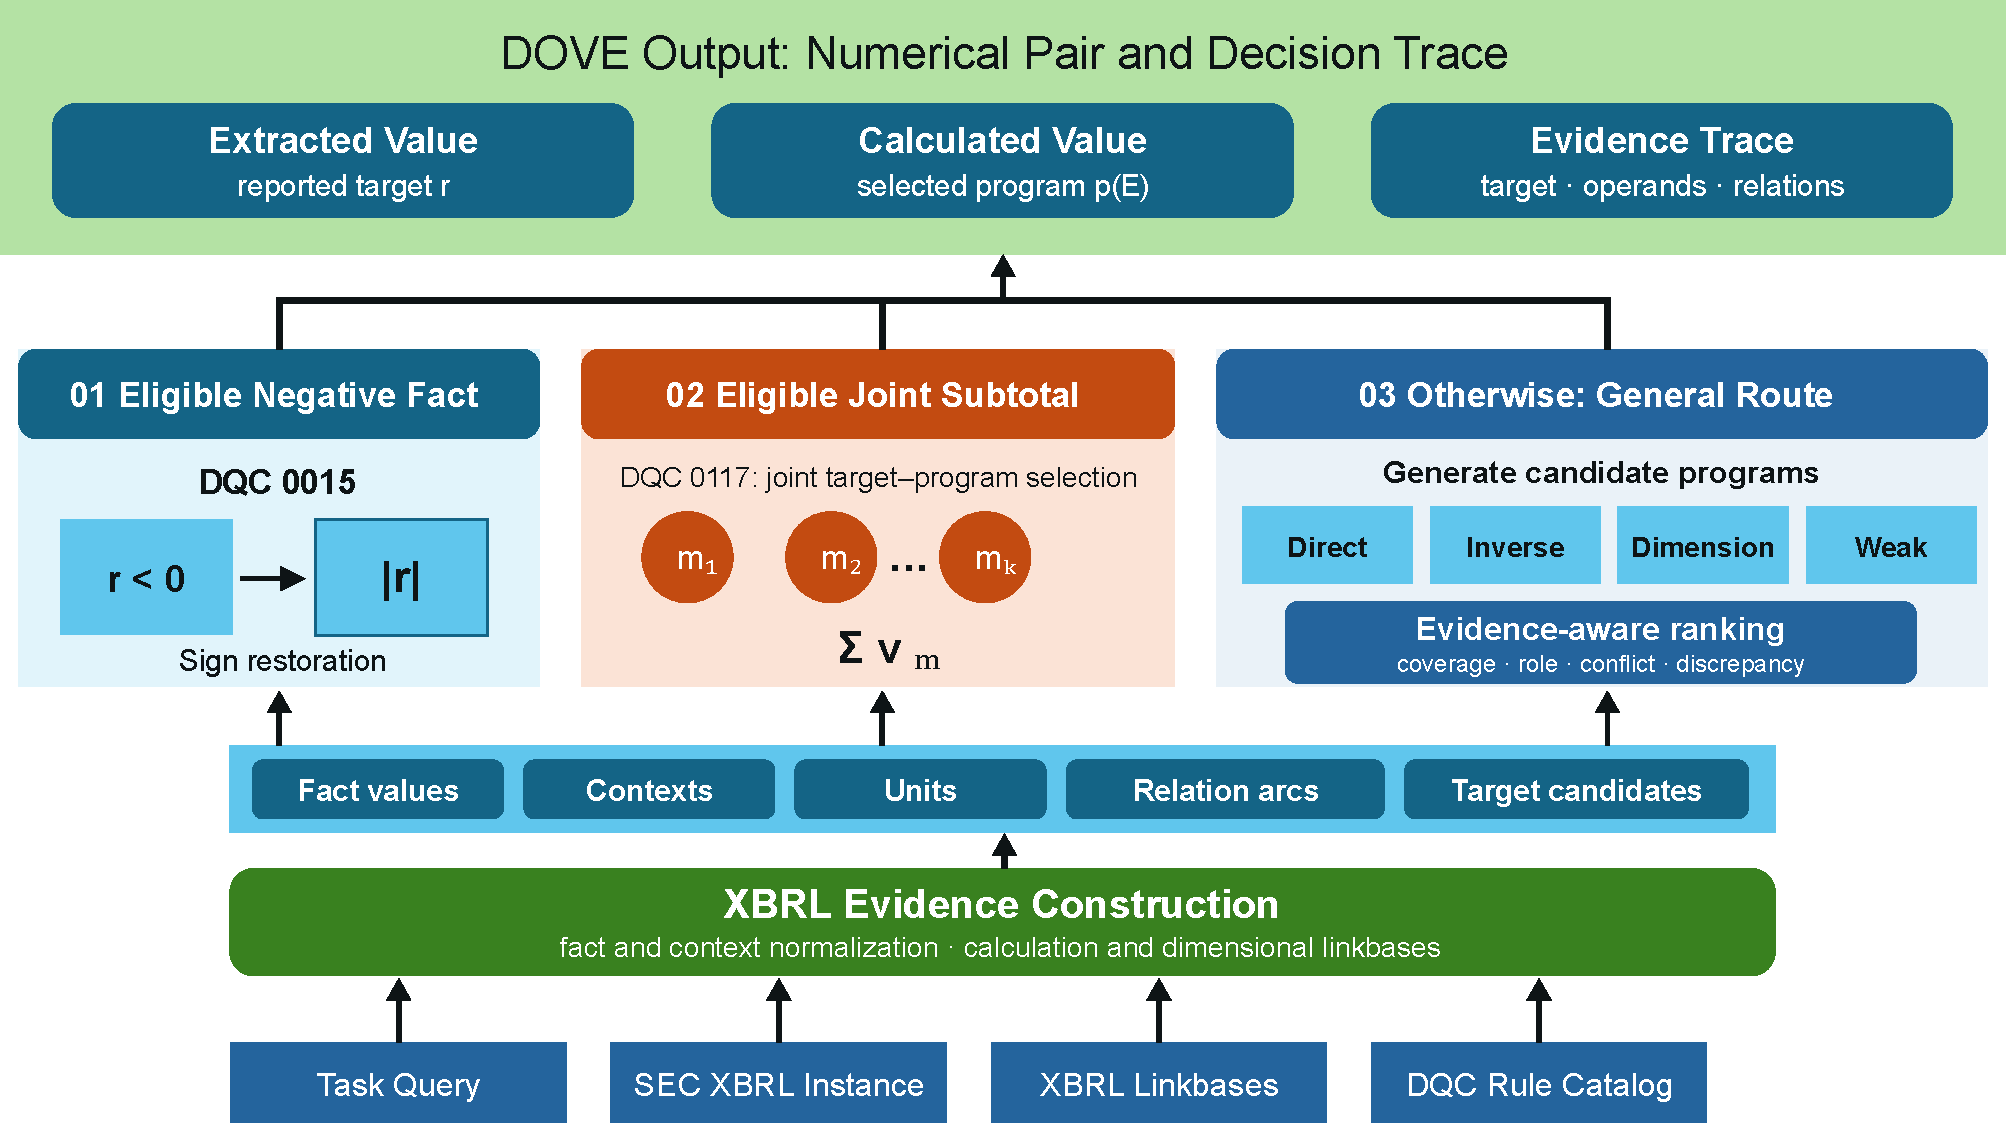
\includegraphics[width=0.98\textwidth]{figures/fig1_dove_architecture_solid.pdf}
\caption{DOVE inference architecture. The system constructs XBRL evidence from the task query, SEC instance, linkbases, and DQC rule catalog. Three prioritized target/program-selection routes lead to the extracted value, calculated value, and an evidence trace containing the selected target, operands, and relations.}
\label{fig:overview}
\end{figure*}

A financial fact is represented as
\begin{equation}
f=(c,v,\tau,u,\delta,\pi),
\end{equation}
where $c$ is the concept, $v$ the Decimal value, $\tau$ the full period, $u$ the unit, $\delta$ the explicit and typed dimensions, and $\pi$ the precision and source metadata. A program candidate is
\begin{equation}
p=(m,\hat y,\mathcal O,\rho,\mathcal M,s),
\end{equation}
where $m$ denotes its program type, $\mathcal O$ its operands, $\rho$ relationship coverage, $\mathcal M$ missing or conflicting evidence, and $s$ its score. Reported observations and computed candidates are stored separately, so execution does not overwrite the filing's values.

\subsection{XBRL Parsing and Comparison Keys}
\label{sec:parsing}

The parser begins with the instance document. It records each non-nil numeric fact, resolves its context and unit references, and normalizes the lexical value to Python \texttt{Decimal}. An instant context is represented by its instant date; a duration context retains both start and end dates. The entity identifier, explicit dimensions, typed dimensions, unit measures, decimals/precision metadata, and document position are retained with the fact.

Calculation linkbases are converted into weighted parent--child arcs grouped by extended-link role. Definition linkbases supply dimensional-domain and domain-member structure. Presentation linkbases provide a weaker ordering and grouping signal when definition evidence is sparse. The solver keeps the role URI with every arc because the same concept can participate in several statement networks with different financial meanings.

For fact comparison, \dove{} combines the context with the fact's unit in a comparison key:
\begin{equation}
K(f)=(e,\tau,u,D_{\mathrm{exp}},D_{\mathrm{typed}}),
\label{eq:comparison-key}
\end{equation}
where $e$ is the entity, $\tau$ the full period, $u$ the normalized unit, and the final two terms are sorted dimension maps. Two operands are directly compatible when their period, unit, and fixed dimensions satisfy the route-specific constraints. Dimensional aggregation relaxes exactly one selected axis while retaining the remaining dimensions.

Duplicate facts used as calculation operands are grouped by concept and comparison key. Where a modal reported precision is available among compatible statement facts, selection prefers that precision, then finer and coarser precision, with source order resolving ties. Equal values provide the same numerical observation; conflicting values are recorded and penalize affected direct candidates. The fact-order experiment in Section~\ref{sec:order} tests the resulting source-order dependence.

\subsection{Context-Aware Target Selection}
\label{sec:selection}

Initial candidates are numeric occurrences of the target concept with a non-null value. They are ranked by period agreement, dimensional sparsity, temporal details, and source order. The comparison key in Eq.~\eqref{eq:comparison-key} is used when matching operands; precision and duplicate handling follow Section~\ref{sec:parsing}.

Period ranking rewards agreement with the requested instant or end date and, when specified, the duration start date. These are ranking features rather than a universal hard period filter. Dimensioned candidates remain available to the specialized selectors. Unit compatibility is enforced during operand collection, keeping facts with different measurement units out of the same program.

Rule-aware selectors refine this ordering through the three prioritized routes.

For DQC~0015-like cases, the solver enumerates negative facts satisfying the concept, requested period, and public rule applicability and exclusion predicates. Equal-value occurrences provide nested-context support when they share concept, entity, full period, and unit, and one dimension map strictly contains the other: every existing axis/member assignment is preserved and at least one additional axis is fixed. Equivalent duplicates are collapsed before this check. Values with such support are preferred; source order selects the first eligible occurrence of a supported value, or the first eligible negative fact if no support exists. This is a scope-selection heuristic.

For DQC~0117-like cases, the joint selector pairs an existing subtotal with an aggregation program over an additional axis. The frozen selector admits subtotals with one eligible explicit dimension and no typed dimensions. Operands preserve that fixed dimension and match the subtotal's entity, full period, and unit. Admitted sums differ from the reported subtotal and have a generator score of at least 0.3. Role support and the generator score determine the joint score; ties use the subtotal's source position. The selected subtotal/program pair is retained as a joint decision.

The general route selects a target first, then pools eligible direct, inverse, sign-recovery, and dimensional programs. For exact-period queries with only dimensioned target occurrences, a qualifying dimensional candidate can activate a virtual unqualified target whose reported output is serialized as zero. This undimensioned computational placeholder allows an aggregate to be reconstructed from disclosed member facts when no corresponding aggregate fact is reported. The zero encodes an absent aggregate under the submission contract, not an observed financial zero. 

\subsection{Multi-Path Numerical Programs}
\label{sec:programs}

\textit{Direct calculation.} When the target is a calculation parent, observed children $P$ and their linkbase weights yield
\begin{equation}
\hat y_{\mathrm{direct}}=\sum_{i\in P}w_i x_i,
\qquad
\rho=\frac{|P|}{|C|},
\label{eq:direct}
\end{equation}
where $C$ is the effective, non-prohibited child set in the selected role. Partial sums remain available, with missing children recorded explicitly; their interaction with discrepancy-aware ranking is tested in Section~\ref{sec:controlled}. An observed zero is an operand. An absent child contributes no observed term to this partial sum and remains missing evidence. Treating its true value as zero requires an explicit applicable rule or independent evidence establishing zero. The output sentinel described in Section~\ref{sec:task} does not supply such evidence.

\textit{Inverse calculation.} For target child $j$ with nonzero weight $w_j$ and observed parent $p$, reuse $C$ for the parent's effective children and $P\subseteq C$ for observed children. The sibling sets are $C_s=C\setminus\{j\}$ and $P_s=P\setminus\{j\}$, giving
\begin{equation}
\hat x_j=\frac{p-\sum_{i\in P_s}w_i x_i}{w_j}.
\label{eq:inverse}
\end{equation}
The inverse candidate's base score uses coverage $\rho=(1+|P_s|)/(1+|C_s|)$ (Eq.~\eqref{eq:score-inverse}). The extra one in both numerator and denominator accounts for the observed parent, which is also a required operand. The condition that triggers the additional inverse-route penalty is specified in Section~\ref{sec:scoring}.

\textit{Sign recovery.} For a negative fact that satisfies the DQC~0015 applicability conditions, the rule-specific program returns
\begin{equation}
\hat y_{\mathrm{sign}}=|\hat r|.
\end{equation}

This magnitude-preserving repair treats the discrepancy as a sign error. The applicability predicates identify eligible negative facts; the absolute-value operation supplies the task-specific repair. The extracted output retains the original sign, and the trace records the selected fact and applicability evidence.

\textit{Dimensional aggregation.} Given an aggregation axis and observed members $M_{\mathrm{obs}}$,
\begin{equation}
\hat y_{\mathrm{dim}}=\sum_{m\in M_{\mathrm{obs}}}
x(c,\tau,u,\delta_m),
\end{equation}
while all other dimensions in the target context remain fixed. Definition relationships provide the strongest member evidence; presentation relationships provide secondary support. Ancestor--descendant checks reduce double counting.

Network-supported candidates use definition relationships, or presentation structure when dimension--domain links are absent. They consider reported root members and a frontier that descends through missing ancestors. A reported ancestor suppresses its descendants, avoiding double counting.

\emph{Weak aggregation} sums observed members compatible in concept, entity, period, unit, and fixed dimensions without requiring an explicit member path. Known ancestor--descendant relationships still suppress overlapping descendants. This alternative is retained when its value is not already produced by a network candidate for the same axis, including when an incomplete network exists. Its base score is 0.38, and its trace records observed-fact provenance and unresolved completeness. This is the component removed in Section~\ref{sec:ablation}.

\subsection{Evidence Scoring and Decision Traces}
\label{sec:scoring}

Candidate scores combine relationship coverage, operand count, statement-role support, and duplicate conflict. The base scores for the direct and inverse programs in Eqs.~\eqref{eq:direct} and~\eqref{eq:inverse} are
\begin{align}
s_{\mathrm{direct}}&=0.76+0.13\rho+0.004\min(n,10)+b-0.05d,
\label{eq:score-direct}\\
s_{\mathrm{inverse}}&=0.72+0.16\rho+0.002\min(n,10),
\label{eq:score-inverse}
\end{align}
where $n$ counts observed children for a direct program and observed siblings, excluding the parent, for an inverse program. The role bonus $b$ is 0.02 when the role description matches a statement-related keyword (statement, balance sheet, income, or cash flow), and zero otherwise. The indicator $d\in\{0,1\}$ is one when any child concept has conflicting compatible fact values. A direct candidate is generated when at least one compatible child operand is found in a calculation role for the selected target. If any role produces such a candidate, every inverse candidate receives a further score penalty of 1.0. The inverse base score is at most 0.90, so this penalty places it below the 0.10 report-copy fallback. Thus, in the ordinary general-route pool, any available direct candidate makes inverse programs ineligible to win, even when the direct candidate is incomplete. This encodes a preference for the target's own parent--child network. A complete inverse equation can nevertheless provide stronger operand support than a partial direct sum. Removing the inverse penalty changes zero Practice outputs, so this comparison supplies no empirical advantage for the route priority. We retain it as a documented property of the submitted heuristic. A completeness-aware extension would qualify both routes before ranking.

A discrepancy preference subtracts 0.60 from a pooled candidate that reproduces the reported value:
\begin{equation}
s'(p)=s(p)-0.60\,\mathbf{1}[\hat y(p)=\hat r].
\label{eq:discrepancy}
\end{equation}
Here $s(p)$ includes the preceding generator and inverse-route adjustments. Dimensional generators subtract 0.25 from report-equal sums before pooling. A report-copy fallback sets the calculated output equal to the selected reported value ($\hat y=\hat r$) and is always appended afterward with score 0.10. In general-route selection, it wins if no program is generated or all adjusted program scores fall below 0.10. These preferences were motivated by the unequal reference pairs in public Practice. Section~\ref{sec:controlled} examines how the same preference affects selection when the report is correct and an incomplete competitor is present.

General-route candidates are ordered by adjusted score using a stable sort. Equal scores retain the order in which generator outputs were added to the pool; within the direct generator, operand count is a secondary key. The joint route ranks subtotal/program pairs internally because it resolves both choices together. It compares the joint score and then the subtotal's source position, and commits the winning pair. The general candidate pool remains available for diagnostics without replacing that joint decision. Thus selection is route-specific, and generation or source order can affect ties (Section~\ref{sec:order}).

The coefficients are fixed development choices; the archived ablations vary the named components while retaining the remaining configuration.

For every output, \dove{} records the target fact and context, selected route, operands and weights, coverage, missing items, duplicate conflicts, candidate scores, and fallback state. These traces support rule-level debugging, component ablation, and reliability testing.

The submission layer writes each identifier and two Decimal-rendered values. Validation checks identifiers, JSON keys, and numeric parseability; diagnostics remain separate.

\section{Experimental Setup}
\label{sec:protocol}

\subsection{Submitted Configuration and Evaluation Scope}
All main analyses use the frozen configuration that produced the accepted Test file. Practice comparisons, component ablations, and reliability audits are post-submission analyses of this frozen solver; later variants are used only for offline diagnostics and do not affect the reported official result. Canonical lexical ordering is an explicitly separate offline variant. Replay checks reproduced all 680 accepted Test pairs and 3,320 prediction records across ten Practice conditions.

\subsection{Data and Input Compatibility}
Table~\ref{tab:data} summarizes the phases. Practice comprises the 332 public FinMR cases from FinAuditing~\cite{wang2026finauditing,task3data}. Development and Test each contain 680 questions with withheld reference answers. Development returns aggregate scores during construction. Test returned acceptance receipts during the competition, and the last valid submission determined the final result~\cite{task3submission}. Rule identifiers are omitted from Development and Test inputs; Section~\ref{sec:selection} describes the solver's route inference.

\begin{table}[t]
\caption{Task 3 Data Phases}
\label{tab:data}
\centering
\small
\begin{tabular}{lrrl}
\toprule
Phase & Cases & Labels & Use in this paper \\
\midrule
Practice & 332 & Public & Baselines and diagnostics \\
Development & 680 & Hidden & Aggregate feedback \\
Test & 680 & Hidden & Official final evaluation \\
\bottomrule
\end{tabular}
\end{table}

Practice contains 110 DQC~0015, 120 DQC~0117, and 102 DQC~0126 cases. All 332 have a flagged inconsistency and unequal reference values~\cite{task3data}. This public-set property motivated the discrepancy preference in Section~\ref{sec:scoring}. It is a development heuristic, not a correctness condition imposed on unseen Test answers or filings that satisfy their accounting relationships.


Practice inputs also have compatibility and reference issues that affect local evaluation. The frozen parser logs XML recovery errors for 248 queries; the remaining 84 form the no-recovery stratum. Separately, 126 queries finish with \texttt{target\_not\_found}. The recovery flag describes parser behavior on the packaged query, rather than the integrity of the original filing.

Seventeen byte-identical query groups cover 47 records with conflicting normalized reference pairs. A query-only deterministic solver cannot distinguish records within these groups. Removing all 47 defines a 285-record no-conflict stratum, which overlaps both parser strata. We retain every record in the primary 332-example evaluation and use the strata to interpret the comparisons.

\subsection{Metrics and Comparisons}
The official Test result uses the organizer's LLM evaluator and published leaderboard~\cite{task3results}. Local Practice evaluation compares Decimal-normalized numerical pairs exactly. A pair is correct only when both values match the reference, and unresolved predictions count as incorrect. Every primary Practice condition uses the same queries, order, denominator, and scoring routine.

The organizer's full rule baseline retains its own parser, target selection, and fallback behavior. Its extraction-only and sign-flip modes supply simpler references. Fixed-extraction controls reuse DOVE's selected reported values, changing only the subsequent numerical operation. DOVE component interventions use the frozen implementation with the named component changed. The $2\times2$ ablation crosses weak aggregation with discrepancy-aware ranking; disabling the latter removes both the 0.60 pooled penalty and the 0.25 dimensional-generator penalty.

The reliability audit measures output changes under fact permutations and selection behavior on constructed complete and incomplete equations. These tests address stability and decision mechanisms. Official performance, local reference agreement, and perturbation stability are reported as distinct measurements. Protocols, seeds, traces, and oracle operands are provided in the public reproduction repository.

\section{Task Performance and Component Analysis}

\subsection{Official Test Performance}

Table~\ref{tab:test} reports the official result. \dove{} answers 655 of 680 examples correctly, reaches 96.32\% accuracy, and ranks joint eighth among 23 listed teams. It solves every DQC~0126 case, while DQC~0117 has the lowest rule-level accuracy, 79.63\%.

\begin{table}[t]
\caption{Official Test Performance}
\label{tab:test}
\centering
\small
\begin{tabular}{lrrr}
\toprule
Rule & Examples & Correct & ACC \\
\midrule
DQC 0015 & 162 & 148 & 91.36\% \\
DQC 0117 & 54  & 43  & 79.63\% \\
DQC 0126 & 464 & 464 & 100.00\% \\
\midrule
Overall  & 680 & 655 & 96.32\% \\
\bottomrule
\end{tabular}
\end{table}

The official error decomposition is SER 0.00\%, EER 1.03\%, and CER 2.65\%. Of the 25 incorrect cases, 14 belong to DQC~0015 and 11 to DQC~0117. Thus DQC~0015 contributes more errors in absolute terms despite its higher accuracy. DQC~0126 comprises 464/680 cases, or 68.24\% of Test.

The joint-first systems, Polymanes and FinVeritas, each obtain 665 correct predictions. Both have the same correct counts as DOVE on DQC~0015 and DQC~0126, and obtain 53 rather than 43 correct DQC~0117 predictions~\cite{task3results}. Their ten-case aggregate advantage is therefore confined to this dimensional rule group. These totals identify the rule-level score difference without revealing which individual predictions differ or establishing their error causes.

\begin{figure*}[t]
\centering
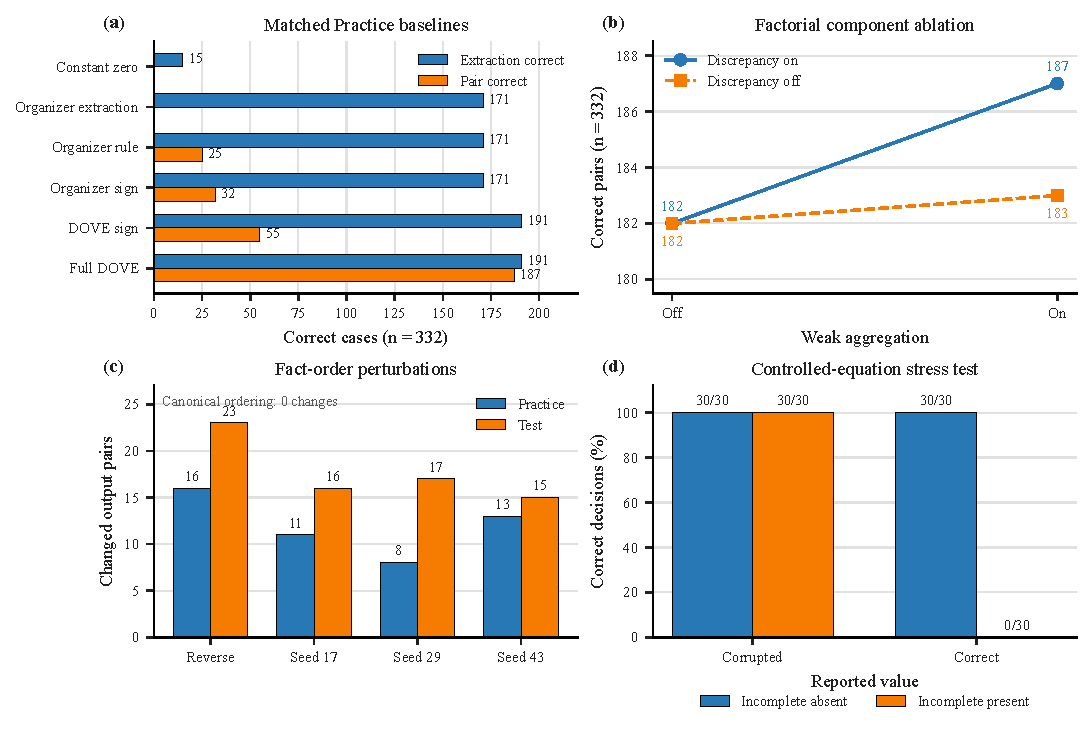
\includegraphics[width=\textwidth]{figures/fig2_empirical_summary_solid.pdf}
\caption{Empirical summary of the labeled and controlled experiments. (a) Matched Practice baselines report exact extraction and pair-correct counts. (b) The $2\times2$ ablation exposes the interaction between weak aggregation and discrepancy-aware ranking. (c) Fact-order perturbations change outputs in the original solver, while canonical ordering yields zero changes in all four trials. (d) Controlled equations isolate the failure induced by a competing incomplete relation. Panels report counts on the fixed evaluation sets and perturbations.}
\label{fig:experiments}
\end{figure*}

\subsection{Matched Practice Baselines}
\label{sec:practice-baselines}

Table~\ref{tab:baselines} and Figure~\ref{fig:experiments}(a) compare the archived Practice conditions. The full solver obtains 187 correct pairs, compared with 25 for the organizer's full rule baseline. DOVE also identifies 191 reported values correctly, compared with 171 for the organizer extractor. This end-to-end comparison includes differences in parsing, target selection, and numerical execution.

\begin{table}[t]
\caption{Matched Practice Results on All 332 Examples}
\label{tab:baselines}
\centering
\footnotesize
\setlength{\tabcolsep}{4pt}
\begin{tabular}{lrr}
\toprule
Condition & Extraction & Pairs \\
\midrule
Constant zero & 15 & 0 \\
Organizer extraction only & 171 & 0 \\
Organizer full rule baseline & 171 & 25 \\
Organizer sign flipping & 171 & 32 \\
DOVE extraction only & 191 & 0 \\
DOVE extraction + sign flipping & 191 & 55 \\
Full \dove{} & 191 & 187 \\
\bottomrule
\end{tabular}
\end{table}

Holding DOVE's reported outputs fixed, sign flipping obtains 55 correct pairs and the full solver obtains 187, a gain of 132 pairs. This comparison isolates the value of the subsequent program execution and selection pipeline from changes in extraction. Among the 191 correctly extracted cases, the full solver also computes the reference value in 187 (97.91\%). Extraction-only modes copy the selected report into the calculated field; they obtain no correct pairs because all Practice reference pairs contain unequal values.

\subsection{Factorial Component Ablation}
\label{sec:ablation}

Figure~\ref{fig:experiments}(b) crosses weak aggregation with discrepancy-aware ranking. The full solver obtains 187 correct pairs; removing weak aggregation alone yields 182, removing the discrepancy preference alone yields 183, and removing both yields 182.

The conditional contribution of weak aggregation is five cases with the preference active and one case without it. The preference contributes four cases with weak aggregation active and zero without it. Candidate construction and ranking therefore contribute jointly: weak aggregation supplies alternatives whose selection depends on the discrepancy preference.

The four cases lost when the discrepancy preference is removed are contained in the five cases lost when weak aggregation is removed. Adding the two single-component losses would therefore double-count four shared cases.

Additional interventions produced identical Practice outputs: removing the nested-context preference, removing joint subtotal selection, removing inverse-route downweighting, and adjusting related admission thresholds. These null interventions narrow the set of components with observed decision impact in the frozen Practice run.

\paragraph{Parameter sensitivity}
The constants in the submitted configuration are development heuristics. The available archive does not establish a held-out procedure for selecting their numerical magnitudes. Retrospective scaling of both equality penalties by $0$, $0.5$, $1$, and $1.5$ yields 183, 185, 187, and 187 correct Practice pairs. Moving the related admission thresholds from 0.3 to 0.1 or 0.5 leaves all Practice outputs unchanged. These measurements describe local sensitivity on the development-exposed split. The aggregate official Test score evaluates the complete frozen policy and cannot isolate parameter or component transfer.

\subsection{Results Across Practice Strata}
\label{sec:practice-diagnostics}

The full solver obtains 79/84 correct pairs in the no-recovery stratum and 108/248 in the recovery stratum. On the 285 records outside conflicting-reference groups, it obtains 181 correct pairs; the remaining six of its 187 full-set correct pairs lie within the conflict groups. These results connect the overall Practice count to the input and reference characteristics established in Section~\ref{sec:protocol}.

The component interaction persists across these diagnostics. On the 84 no-recovery cases, removing weak aggregation loses three correct pairs and removing the discrepancy preference loses two. All five cases affected by the full-set ablation lie outside the conflicting-reference groups. Appendix~\ref{app:strata} gives the full stratified ablation.

\section{Reliability Audit}
\label{sec:reliability}

\subsection{Test Execution-Path Audit}

The frozen traces identify 467 direct calculation programs, one inverse program, 162 sign programs, 43 network-supported dimensional programs, and seven unlinked observed-member aggregations. No Test prediction selects the report-copy fallback defined in Section~\ref{sec:scoring}, and all 680 queries produce parseable output pairs.

Every selected direct or inverse program has an explicit relation and observed operands. The local completeness check classifies 362 of these 468 paths as complete and records missing terms for 106. Among the 50 dimensional paths, 22 pass the check and 28 retain incomplete or unresolved coverage. Appendix~\ref{app:coverage}, Table~\ref{tab:coverage}, gives the route-specific criteria. These program-level diagnostics measure operand coverage, while Table~\ref{tab:test} reports correctness by official rule group. Missing operands motivate the controlled selection audit in Section~\ref{sec:controlled}; local coverage alone does not determine numerical correctness.

\subsection{Fact-Order Sensitivity}
\label{sec:order}

We reverse the parsed facts or permute them using seeds 17, 29, and 43, preserving their multiset, contexts, units, and relationship networks. Figure~\ref{fig:experiments}(c) reports changed output pairs. Across these four perturbations, the submitted configuration changes 8--16 Practice outputs and 15--23 Test outputs.

A diagnostic counterfactual applies canonical lexical ordering before target selection; it is separate from the submitted configuration. It produces no output changes under the tested permutations and obtains 186 correct Practice pairs, one fewer than the submitted configuration. Relative to the accepted Test file, it changes 18 numerical pairs. The official score applies to the submitted file; the 18 changed pairs have no separate official score.

Source order participates in target and duplicate selection and affects candidate ordering, providing mechanisms for the observed dependence. Canonical lexical ordering removes this dependence under the tested fact permutations, while its Practice trade-off separates stability from reference agreement. The audit covers fact permutations with the remaining XML evidence fixed.

\paragraph{Which cases change}
Replaying all four permutations gives a union of 23 changed Test cases. Inspection of target identities yields 19 cases selecting among multiple eligible negative facts, two cases selecting between tied dimensional subtotals, and two cases selecting unequal values in the same semantic context and unit. In the last two cases, precision intervals overlap. For example, TEST3\_000165 contains 3,979,000 with decimals $-3$ and 4,000,000 with decimals $-5$. Thus raw inequality alone does not establish inconsistent duplicates. We observe no changed case having a unique eligible target value under the implemented checks. Establishing uniqueness from fuller XBRL semantics remains open.

Representative reversals expose distinct mechanisms. TEST3\_000002 switches from context c-127, reporting $-1{,}535{,}000$, to c-11, reporting $-2{,}184{,}000$; both satisfy the negative-fact selector, and each output applies sign recovery. TEST3\_000165 keeps c-1 and its computed value 14,500,000 while changing the reported value from 3,979,000 to 4,000,000. TEST3\_000198 switches from ServiceAndFeeRevenuesMember to InterestIncomeLoansMember at the same joint score 0.8038, changing the output pair from $(475{,}279{,}000,9{,}168{,}000)$ to $(9{,}143{,}000,1{,}818{,}000)$. The released traces identify all 23 cases and their outputs under each permutation.

These cases motivate precision-aware duplicate resolution and semantic scope qualification before source-order tie breaking. The supplied queries and implemented predicates admit alternatives in these cases. Lexical ordering makes a reproducible choice among them, while correctness requires additional evidence about the intended scope. Per-case official Test references are unavailable, so the traces establish the mechanism and leave the relative correctness of these alternatives unresolved.

\subsection{Controlled Complete and Incomplete Equations}
\label{sec:controlled}

The archived controlled experiment contains 120 equations, with 30 examples in each of four conditions: C1 (correct report, no competing equation), C2 (corrupted report, no competing equation), C3 (correct report, incomplete competitor), and C4 (corrupted report, incomplete competitor). Every condition includes a complete relation,
\begin{equation}
y=a+wb,\qquad w\in\{-1,1\},
\end{equation}
and an independent rational-number oracle computes $y$. The reported value is either $r=y$ or a corrupted $r=y+\delta$, $\delta>0$. Competing conditions add a second relation $y=c+d$ but expose only $c=y+\delta$, yielding an incomplete partial sum. This construction makes the partial sum agree with the corrupted report and disagree with the correct report, isolating the effect of the agreement penalty on the candidate ordering.

Figure~\ref{fig:experiments}(d) shows that \dove{} retains all 30 correct reports in C1 and repairs all 60 corrupted reports in C2 and C4. In C3, the incomplete competitor causes all 30 correct targets to be changed incorrectly.

The ranking reversal follows Eq.~\eqref{eq:discrepancy}. With a corrupted report $r=y+\delta$, the incomplete partial sum $c$ equals the report and receives the agreement penalty, while the complete result $y$ does not; the complete relation wins in C4. With a correct report $r=y$, the complete relation receives the penalty, while the discrepant partial sum does not and ranks above it in C3. Without that competitor, the complete program remains selected in C1 despite the penalty. The resulting failure is a selection error: the complete program computes the oracle value, but its agreement with a correct report lowers its rank. Together with the Practice ablation, this explains the trade-off in the discrepancy preference. It helps select correct alternatives in the flagged Practice cases while overturning correct reports in this controlled configuration.

\section{Discussion}

\subsection{Task Performance and Scope Resolution}
The ten-case aggregate gap to the leading systems lies in DQC~0117. Dimensional execution requires both a subtotal scope and an adequate member partition. DOVE makes these choices explicit through its joint selector and aggregation programs, connecting each numerical output to the selected scope and member evidence.

A dimensional extension should establish the target's fixed scope, verify that members are disjoint and collectively cover the aggregate, and distinguish omitted members from reported zero values. The 28 incomplete or unresolved dimensional paths are local coverage diagnostics. Their relationship to the 11 official DQC~0117 errors cannot be determined from aggregate labels alone.

The Practice ablation identifies weak aggregation and discrepancy-aware ranking as interacting components. Other selector interventions leave Practice outputs unchanged. The measured component gains are thus concentrated in the construction and selection of aggregation alternatives.

\subsection{Reliability of Selection Decisions}
\label{sec:qualification}
The audits distinguish two failures. Fact-order sensitivity arises from target, duplicate, and candidate tie resolution. Canonical lexical ordering removes output variation under the tested permutations, with a one-pair decrease in Practice accuracy. This separates stability from agreement with task references: a stable decision rule can choose a different numerical pair.

Incomplete-candidate promotion arises from the ranking objective. In the controlled equations, the complete relation remains available and computes the correct value, yet the discrepancy preference favors an incomplete alternative when the report is correct. The same preference contributes four correct Practice pairs when weak aggregation is active. Its benefit therefore depends on the task's discrepancy setting and the competing evidence.

The audits motivate stable fact/context tie resolution and evidence qualification before discrepancy-based ranking. Such an extension would check rule and context eligibility, relationship provenance, operand coverage, and dimensional closure before numerical preferences. The existing traces expose the operands and missing evidence for this investigation.

\subsection{Limitations}
\textit{Development-set dependence.} Practice informed development, all 332 reference pairs contain discrepancies, and the post-submission baselines and ablations reuse this split. Also, 248 queries trigger XML recovery and 47 records belong to identical-query groups with conflicting references. These diagnostics characterize the frozen solver and provide limited evidence of transfer to new filings.

\textit{Restricted Test visibility.} Official results provide overall and rule-level counts without per-case reference values. Consequently, changes under permutations cannot be labeled as improvements or regressions, and the dimensional score gap cannot be assigned to particular selection errors. The official LLM evaluator and local exact Decimal-pair scorer use different matching procedures.

\textit{Coverage and external validity.} DOVE implements a subset of XBRL context and dimensional semantics. Some selected calculations retain missing operands or unresolved member coverage. The controlled equations isolate one selection failure without estimating its prevalence in real filings. Task~3 evaluates predefined pairs. Independent replication by other researchers remains to be established.

\subsection{Code and Reproduction Materials}
\label{sec:release}
Code and experiment materials are available at \url{https://github.com/Zhao0335/DOVE}. The release contains the frozen predictor, rule-resource provenance, offline runners, Practice outputs and per-case diagnostics, perturbation seeds, 23 derived Test change traces, and all 120 synthetic queries with rational-number oracle operands. Benchmark inputs are obtained separately from the organizers. Fresh local runs reproduce the ten Practice conditions and all four controlled-equation counts. Source and input hashes identify the evaluated artifacts. The release documents canonical ordering as an offline variant and retains the official score of the submitted policy.

\section{Conclusion}
DOVE achieves 655/680 correct Test answers in FinReason Cup 2026 Task~3, including all DQC~0126 cases. Matched Practice comparisons establish the contribution of numerical execution beyond sign flipping, and factorial ablation identifies the interaction between weak aggregation and discrepancy-aware ranking. Reliability audits expose fact-order dependence and incomplete-candidate promotion. Together, these results connect competition performance to the selection mechanisms that support it and show where exact execution still depends on the quality of the selected evidence.

\appendices

\section{Local Evidence Coverage}
\label{app:coverage}

\begin{table}[h]
\caption{Local Evidence Completeness by Route Family}
\label{tab:coverage}
\centering
\small
\begin{tabular}{lrrr}
\toprule
Route family & Total & Complete & Incomplete \\
\midrule
Direct/inverse & 468 & 362 & 106 \\
Dimensional & 50 & 22 & 28 \\
Sign recovery & 162 & 162 & 0 \\
\bottomrule
\end{tabular}
\end{table}

Completeness in Table~\ref{tab:coverage} is a local solver diagnostic. For calculation paths it requires the expected operands of the selected relation to be observed in compatible contexts: children for a direct program, or the parent and siblings for an inverse program. For dimensional paths it requires the selected member frontier to pass the implemented closure test. Sign recovery is complete when its rule applicability record is present.

\section{Practice Stratification}
\label{app:strata}

Table~\ref{tab:strata} reports correct pairs for the strata defined in Section~\ref{sec:practice-diagnostics}. Column denominators are 332, 84, 248, and 285, respectively.

\begin{table}[h]
\caption{Practice Results by Diagnostic Stratum}
\label{tab:strata}
\centering
\scriptsize
\setlength{\tabcolsep}{3.0pt}
\begin{tabular}{lrrrr}
\toprule
Strategy & All & No rec. & Rec. & No conflict \\
\midrule
Full \dove{} & 187 & 79 & 108 & 181 \\
No weak aggregation & 182 & 76 & 106 & 176 \\
No discrepancy preference & 183 & 77 & 106 & 177 \\
Neither component & 182 & 76 & 106 & 176 \\
\bottomrule
\end{tabular}
\end{table}

\bibliographystyle{IEEEtran}
\bibliography{references}

\end{document}
